%%%%%%%%%%%%%%%%%%%%%%%%%%%%%%%%%%%%%%%%%%%%%%%%%%%%%%%%%%%%%%%%%%%%%%%%%
% Chapter Guidelines
%%%%%%%%%%%%%%%%%%%%%%%%%%%%%%%%%%%%%%%%%%%%%%%%%%%%%%%%%%%%%%%%%%%%%%%%%

\chapter{Recommandations}
\label{cha:guidelines}

Voici quelques règles et recommandations CEA pour l’écriture de votre mémoire :

\begin{enumerate}
    \item Règles de confidentialité : Les informations que vous avez pu récolter durant votre temps au CEA peuvent être confidentielles. Merci de vous rapprocher de votre tuteur de stage pour les connaître. Apposez une mention \textit{Confidentiel} sur la première page de votre document ainsi qu’à chaque page qui le nécessite (en-tête ou pied de page) le cas échéant. Pour rappel : voir Figure~\ref{fig:scheme_confidential}. Plus de détails sont donnés dans le \href{https://doc-dssn.intra.cea.fr/Documents partages/Referentiel_DSSN/10_Protection_contre_les_actes_de_malveillance/PAM_10_Protection_des_informations_et_du_patrimoine_scientifique_et_technique_du_CEA/Guide_protection_de_l_information.pdf}{guide de protection de l’information}.

\begin{figure}[h]
    \centering
    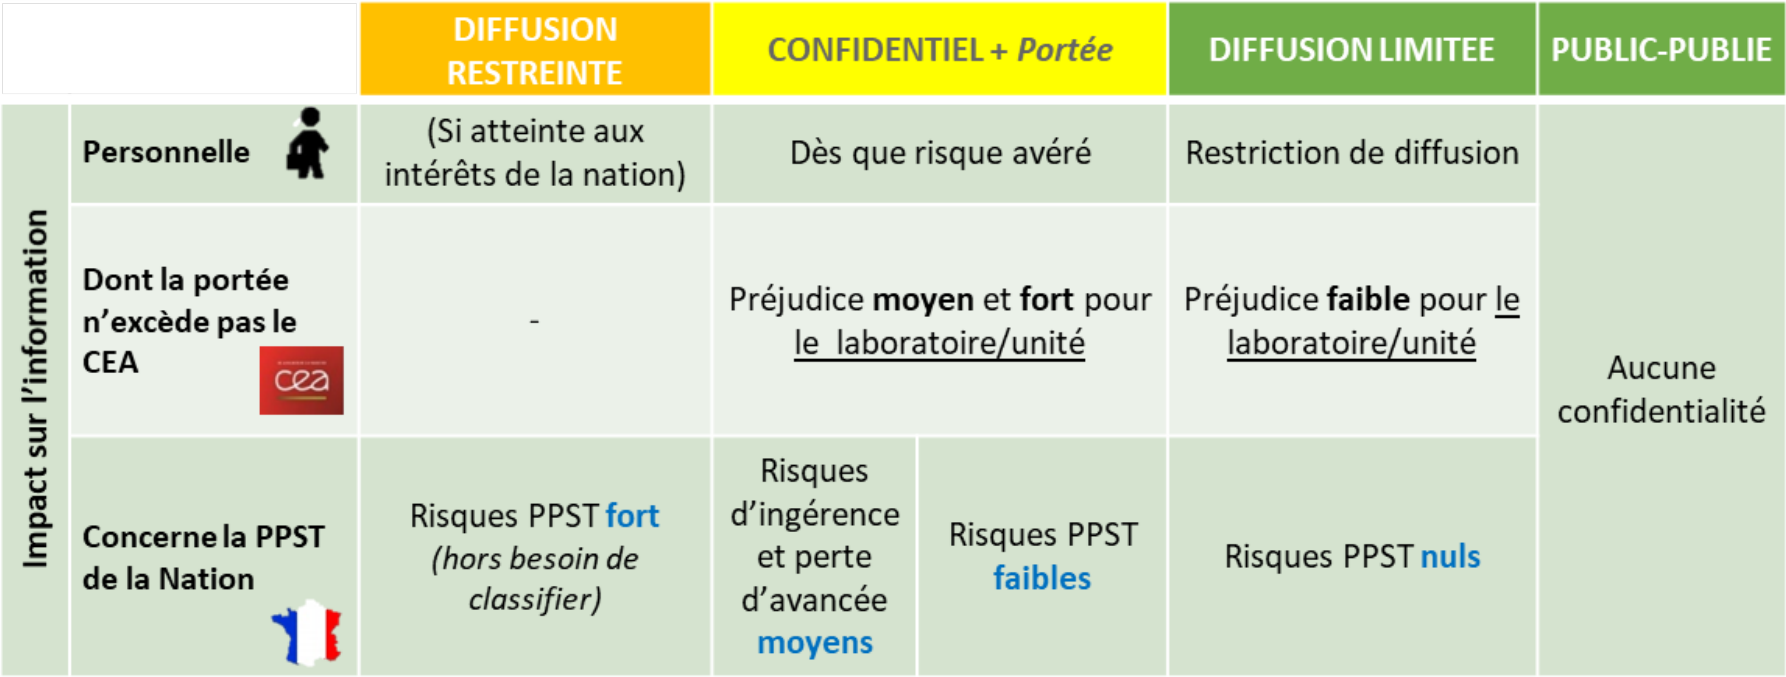
\includegraphics[width=\linewidth]{Chapter_Guidelines/Figures/Schéma_confidentialité.png}
    \caption{Les niveaux de protection de l’information en fonction de leur sensibilité}
    \label{fig:scheme_confidential}
\end{figure}

    \item Propriété intellectuelle : \textbf{Une vigilance importante} doit être apportée à \textbf{toutes informations scientifiques diffusées} dans le cadre de votre mémoire ET de votre soutenance, qui ne soient pas déjà dans le domaine public. La diffusion d’information brevetable, dans un cadre non confidentiel, peut être motif d’une demande de brevet non recevable. Si cela vous concerne, vous pouvez signer un NDA (accord de confidentialité) avec votre école. Pour la soutenance, soyez vigilant au tiers qui peuvent être présents et qui n’auraient pas signé de NDA.
    \item Médiathèque : Pour vous aider dans l’illustration de votre rapport et dans la description du CEA, une médiathèque est disponible sur l’intranet : \href{https://portail.intra.cea.fr/multimedia}{La médiathèque - Accueil (cea.fr)}
    \item Sources et bibliographies : Pour éviter toute forme de plagiat (c’est une faute grave !), vous devez citer les auteurs et les œuvres dont s’est nourrie votre réflexion.
    \item Intégrité scientifique et règles : Le CEA a adhéré au code de conduite européen pour l’intégrité en recherche. Consultez le sur \href{https://allea.org/code-of-conduct/}{allea.org}.
    \item Recommandation d’écriture : Alignement en Justifié, annotez et recensez tous vos graphiques et schémas avec un titre et légendes, numérotez vos pages. Pour la rédaction des livrables, voir quelques conseils \href{https://www.sciencespo-lille.eu/sites/default/files/guide_preparer_et_rediger_un_memoire_de_recherche.pdf}{ici}, p9-10.
    \item Sauvegarde et archive :
    \begin{itemize}
        \item Pensez à sauvegarder votre mémoire en cours d’écriture sur un réseau CEA, il serait dommage de tout perdre si votre PC vennait à rendre l’âme !
        \item Pour la sauvegarde de la version définitive, merci de vous rapprocher de votre tuteur. Ne la laissez pas dans vos dossiers personnels du PC, qui seront supprimés à votre départ. Il en va de même pour vos travaux.
    \end{itemize}
\end{enumerate}

\clearpage